
\lecture{2}{The Statistical Basis of Thermodynamics}{Qiang Zhu}{scribe-name1,2,3}
%\footnotetext{These notes are partially based on those of Nigel Mansell.}
% **** YOUR NOTES GO HERE:
% Some general latex examples and examples making use of the
% macros follow.  
%**** IN GENERAL, BE BRIEF. LONG SCRIBE NOTES, NO MATTER HOW WELL WRITTEN,
%**** ARE NEVER READ BY ANYBODY.

\section{Microstates and Macrostates}
We consider a system composed of $N$ identical particles confined to a space of $V$.
The total energy $E$ would be equal to the sum of the energies of the individual particles.
\begin{equation} E = \sum_i n_i\epsilon_i \end{equation}

The specification of the actual values of the parameters $N, V, E$ then defines a $macrostate$ of the system.
At the molecular level, however, a large number of possibilities still exist because at that level there will be a large number of different ways to make the total state of $N,V,E$ (think out arranging the coins with different sequence of head and tail).
Each of the different ways specifies a $microstate$ or $complexion$ of the given system.

The actual number of all possible microstates ($\Omega$) will be a function of $N, V, E$. In principle, it is from the magnitude of the number of $\Omega$ and from its dependence on the parameters $N, V, E$, that complete thermodynamics can be derived.


\section{Multiplicity in Einstein Solids}
$N$: Number of the oscillators.\\
$q$: Number of energy states.

\begin{equation}
 \Omega(N, q) = \binom{q+N-1}{q} = \frac{(q+N-1)!}{q!(N-1)!}
\end{equation}

It can be simply proved as follows\\
$q$ circles; \\
$N-1$ vertical lines;\\
how to arrange them? \\
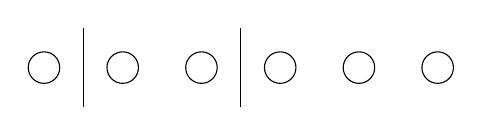
\begin{tikzpicture}
\draw (2,0) circle (0.2cm);
\draw (2.5,-0.5) -- (2.5,0.5);
\draw (3,0) circle (0.2cm);
\draw (4,0) circle (0.2cm);
\draw (4.5,-0.5) -- (4.5,0.5);
\draw (5,0) circle (0.2cm);
\draw (6,0) circle (0.2cm);
\draw (7,0) circle (0.2cm);
\end{tikzpicture}

{\bf Exercises}\\
Calculate the multiplicity of an Einstein solid with 5 oscillators and [1,2,3,4,5] units of Energy.\\
\begin{tabular}{c|c }
$q$ &$\Omega(5,q)$ \\\hline
 1     &  \\
 2     &  \\
 3     &  \\
 4     &  \\
 5     &  \\\hline
\end{tabular}



\section{Contact between statistics and thermodynamics}

\begin{figure}[h]
\centering
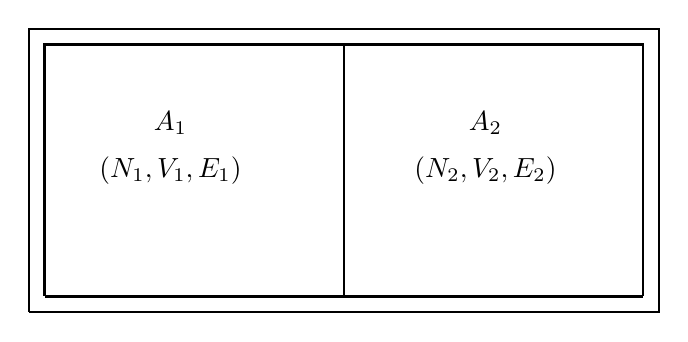
\begin{tikzpicture}[thick]
\draw (0,0.4) -- (8,0.4) -- (8,4) -- (0,4) -- (0,0.4);
\draw (0.2,0.6) -- (4.0,0.6) -- (4.0,3.8) -- (0.2,3.8) -- (0.2,0.6);
\node at (1.8,2.8) {$A_1$};
\node at (1.8,2.2) {($N_1, V_1, E_1$)};
\draw (7.8,0.6) -- (4.0,0.6) -- (4.0,3.8) -- (7.8,3.8) -- (7.8,0.6);
\node at (5.8,2.8) {$A_2$};
\node at (5.8,2.2) {($N_2, V_2, E_2$)};
%\draw [->,decorate,decoration=snake] (3.2,2) -- (4.8,2) node [above, xshift=-1cm]{1500 J};
\end{tikzpicture}
\caption{A schematic of two physical systems in thermal contact.}
\end{figure}

Let's first figure out how $\Omega$ is related to the thermodynamic quantities. We consider two physical systems, $A_1$ and $A_2$, which are separately in equilibrium. Let the macrostate of $A_1$ be represented by the parameters $N_1$, $V_1$and $E_1$ so that it has $\Omega_1(N_1, V_1, E_1)$ possible microstates, and the macrostate of $A_2$ be represented by $\Omega_2(N_2,V_2, E_2)$. Can we derive some thermodynamic properties from $\Omega_1(N_1, V_1, E_1)$ and $\Omega_2(N_2, V_2, E_2)$?

Let's bring two systems into thermal contact. For simplicity, we only allow the heat exchange between the two, while $N$, $V$ remain fixed. This means there could be some interchanges between $E_1$ and $E_2$, however, it has to be restricted by the conservation law.
\begin{equation} E = E_1 + E_2 = \textrm{const} \end{equation}

From the microscopic view,  the total number of microstates could be expressed as,
\begin{equation} \Omega_1(E_1)\Omega_2(E_2) = \Omega_1(E_1) \Omega_2(E-E_1)  \end{equation}

When the system approaches to the equilibrium, what should be the value of $\bar{E_1}$. 
According to the 2nd law, the entropy should reach the maximum. Mathematically, we need to find $\bar{E_1}$ which satisfies,

\begin{equation} 
	\bigg(\frac{\partial {\Omega_1(E_1)}} {\partial {E_1}}\bigg) _{E_1=\bar{E_1}} \Omega_2(E_2) + 
	\bigg(\frac{\partial {\Omega_2(E_2)}} {\partial {E_2}}\bigg) _{E_2=\bar{E_2}} \frac{\partial{E_2}}{\partial{E_1}}\Omega_1(E_1) = 0 
\end{equation}

Remember that $\Delta E_1 = \Delta E_2$ at each time interval, therefore
\begin{equation} 
	\bigg(\frac{\partial {\ln \Omega_1(E_1)}} {\partial {E_1}}\bigg) _{E_1=\bar{E_1}} =
	\bigg(\frac{\partial {\ln \Omega_2(E_2)}} {\partial {E_2}}\bigg) _{E_2=\bar{E_2}}
\end{equation}

Thus, our condition for equilibrium reduces to the equality of parameter $\beta_1$ and $\beta_2$:
\begin{equation} 
	\beta \equiv \bigg(\frac{\partial {\ln \Omega(E)}} {\partial {E}}\bigg) _{E=\bar{E}}
\end{equation}

or a more complete version as follows,
\begin{equation} \label{e1}
	\beta \equiv \bigg(\frac{\partial {\ln \Omega(N,V,E)}} {\partial {E}}\bigg) _{N,V,E=\bar{E}}
\end{equation}

Therefore, we find when two systems are into thermal contact, the exchange of heat continues until the equilibrium $E_1$, $E_2$ reach some values.
This happens only when the respective values of $\beta_1$ and $\beta_2$ become equal. It is then natural to expect that the parameter $\beta$ is somehow related to $T$. To determine this relationship, we recall the thermodynamic formula
\begin{equation} \label{e2}
	\bigg(\frac{\partial S}{\partial E}\bigg)_{N,V} = \frac{1}{T}
\end{equation}

Comparing eq. \ref{e1} and \ref{e2}, we find
\begin{equation} 
	\bigg(\frac{\Delta S}{\Delta \textrm{ln} \Omega} \bigg) = \frac{1}{\beta T} = \textrm{const}
\end{equation}

This correspondence was firstly established by Boltzmann. It was Planck who first wrote the explicit formula
\begin{equation}
	S = k\textrm{ln}\Omega
\end{equation}
It means that the absolute value of the entropy of a given physical system in terms of the total number of microstates accessible to it conformity with the given macrostate, which provides a bridge between micro and macroscopic.


\section{More complete contact}
Let's continue to examine a more elaborate exchange between $A_1$ and $A_2$.

not only,
\begin{equation} 
	\bigg(\frac{\partial {\textrm{ln} \Omega_1(E_1)}} {\partial {E_1}}\bigg) _{E_1=\bar{E_1}} =
	\bigg(\frac{\partial {\textrm{ln} \Omega_2(E_2)}} {\partial {E_2}}\bigg) _{E_2=\bar{E_2}}
\end{equation}
but also
\begin{equation} 
	\bigg(\frac{\partial {\textrm{ln} \Omega_1(V_1)}} {\partial {V_1}}\bigg) _{V_1=\bar{V_1}} =
	\bigg(\frac{\partial {\textrm{ln} \Omega_2(V_2)}} {\partial {V_2}}\bigg) _{V_2=\bar{V_2}}
\end{equation}

Our conditions for equilibrium now take the form of an equality between the pair of ($\beta$, $\eta$)
\begin{equation} 
	\eta \equiv \bigg(\frac{\partial {\textrm{ln} \Omega(N,V,E)}} {\partial {V}}\bigg) _{N,E,V=\bar{V}}
\end{equation}

Similarly, there might be exchanges between particles, while need another parameter $\zeta$,
\begin{equation} 
	\zeta \equiv \bigg(\frac{\partial {\textrm{ln} \Omega(N,V,E)}} {\partial {N}}\bigg) _{V,E,N=\bar{N}}
\end{equation}

To determine the physical meaning of the parameters $\eta$ and $\zeta$, we make use of the thermodynamic identity.
\begin{equation} 
	dE = TdS - PdV + \mu dN
\end{equation}

so
\begin{equation} 
	\begin{split}
	\beta &= \frac{1}{kT} \\
	\eta  &= \frac{P}{kT} \\
	\zeta &= -\frac{\mu}{kT}
	\end{split}
\end{equation}

From the macroscopic view, the equilibrium is reached when
\begin{equation} 
	\begin{split}
	T_1 &= T_2 \\
	P_1 &= P_2 \\
	\mu_1 &= \mu_2 
	\end{split}
\end{equation}

This is identical to the ones following from statistical considerations.
The evaluations of $P$, $\mu$, $T$ indeed requires that energy $E$ be expressed as a function of $N,V,E$,
this should, in principle be possible once $S$ is known.

For instance,
\begin{equation} 
	\begin{split}
		\bigg(\frac{\partial S}{\partial E}\bigg)_{N,V} &= \frac{1}{T} \\
		\bigg(\frac{\partial S}{\partial V}\bigg)_{N,V} &= \frac{P}{T} \\
		\bigg(\frac{\partial S}{\partial N}\bigg)_{N,V} &= \frac{-\mu}{T} 
	\end{split}
\end{equation}


The rest of thermodynamic quantities follow straightforwardly.
\begin{equation}
	\begin{split}
		F &= E - TS \\
		G &= F + PV = E - TS - PV = \mu N \\
		H &= E + PV = G + TS
	\end{split}
\end{equation}
\begin{equation}
	\begin{split}
		C_V &= T(\frac{\partial S}{\partial T})_{N,V} = (\frac{\partial E}{\partial T})_{N,V}\\
		C_P &= T(\frac{\partial S}{\partial T})_{N,P} = (\frac{\partial H}{\partial T})_{N,P}
	\end{split}
\end{equation}

%\section{Homework}
%Problem 3.5, 3.8, 3.11, 3.14, 3.16

